\section{Use Case}
\subsection{\texorpdfstring{{Utente non Loggato}}{Utente non Loggato}}
    Di seguito i requisiti associati all'utente prima di effettuare l'accesso al sistema. In questa fase l'utente ha a disposizione le seguenti funzionalità:
    \begin{itemize}
        \item \textbf{RFO}: Cambio Lingua
        \item \textbf{RF1}: Effettuare Login 
    \end{itemize}
    \begin{figure}[H]
        \centering
        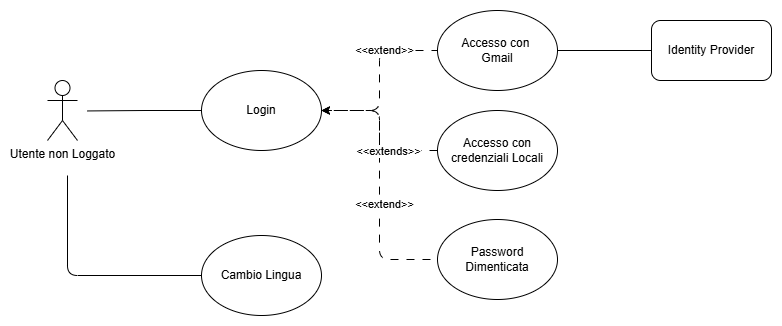
\includegraphics[width=1\textwidth]{../images/UseCase_diagram/useCaseDiagram-USE_CASE2.drawio.png}
        \caption{\textit{Use Case Diagram} - Funzionalità Utente non Loggato}
    \end{figure}
    \subsection*{\textit{Use Case} RFO : Cambio Lingua}
        \subsubsection*{Riassunto}
            Questo \textit{Use Case} descrive come l'utente adatta l'interfaccia alla propria lingua di preferenza prima ancora di effettuare l'accesso, garantendo un'esperienza localizzata.
        \subsubsection*{Descrizione}
            \begin{enumerate}
                \item L'utente seleziona la lingua desiderata (ad esempio inglese, italiano o tedesco) dal menù a tendina presente nell'interfaccia iniziale.
                \item Il sistema riceve la richiesta e aggiorna immediatamente la localizzazione di tutte le stringhe di testo a schermo interrogando i cataloghi di traduzione esterni.
            \end{enumerate}
        \subsubsection*{Eccezioni}
            \begin{enumerate}
                \item Nel caso in cui il catalogo delle traduzioni per la lingua scelta non sia temporaneamente raggiungibile, il sistema mantiene la lingua di default (Inglese) e mostra un avviso temporaneo.
            \end{enumerate}
    \subsection*{\textit{Use Case} RF1: Effettuare Login}
        \subsubsection*{Riassunto}
            Questo \textit{Use Case} descrive come l'utente (Amministratore Comunale o Operatore Tecnico) può accedere al sistema informatico, autenticandosi tramite credenziali locali oppure utilizzando l'autenticazione federata con account Google.
        \subsubsection*{Descrizione}
            \begin{enumerate}
                \item L'utente apre l'applicazione web tramite il proprio browser e il sistema mostra la schermata iniziale contenente la maschera di login.
                \item L'utente sceglie la modalità di accesso preferita; in caso di credenziali locali inserisce email e password, mentre in caso di Google clicca sul pulsante dedicato e viene reindirizzato al sistema \texttt{SSO} esterno.
                \item Una volta che il sistema riceve le credenziali valide o la conferma di avvenuta autenticazione esterna, identifica il ruolo specifico dell'utente (Amministratore o Operatore).
                \item Il sistema completa il processo reindirizzando l'utente alla dashboard principale corrispondente alle autorizzazioni del suo ruolo.
            \end{enumerate}
        \subsubsection*{Estensioni}
            \begin{enumerate}
                \item \textbf{Accesso con Google / Credenziali Locali:} L'utente può scegliere dinamicamente quale provider di identità utilizzare.
                \item \textbf{Password dimenticata:} L'utente clicca sul link di recupero per avviare la procedura di ripristino della propria parola chiave tramite email.
            \end{enumerate}
        \subsubsection*{Eccezioni}
            \begin{enumerate}
                \item Nel caso in cui le credenziali locali inserite siano errate o non registrate, il sistema mostra un messaggio di errore a schermo e richiede di riprovare l'inserimento.
                \item Nel caso in cui l'autenticazione esterna con Google fallisca, il sistema intercetta l'errore e riporta l'utente alla schermata di partenza bloccando l'accesso.
            \end{enumerate}
\newpage
\subsection{\texorpdfstring{{Amministratore e Operatore Tecnico - Visualizzazione e Analisi}}{Amministratore e Operatore Tecnico - Visualizzazione e Analisi}}
    Di seguito i requisiti relativi all'osservazione dei dati ambientali, sia in diretta streaming che consultando i trend passati. Verranno trattati i seguenti Use Case:
    \begin{itemize}
        \item \textbf{RF1}: Logout 
        \item \textbf{RF2}: Visualizzazione Dashboard Generale 
        \item \textbf{RF3}: Visualizzazione Dashboard di Ricerca Edifici 
        \item \textbf{RF4}: Visualizzare Dettagli Edificio 
        \item \textbf{RF4}: Visualizzare Storico Dati 
        \item \textbf{RF8}: Monitoraggio in Tempo Reale 

    \end{itemize}
    \begin{figure}[H]
        \centering
        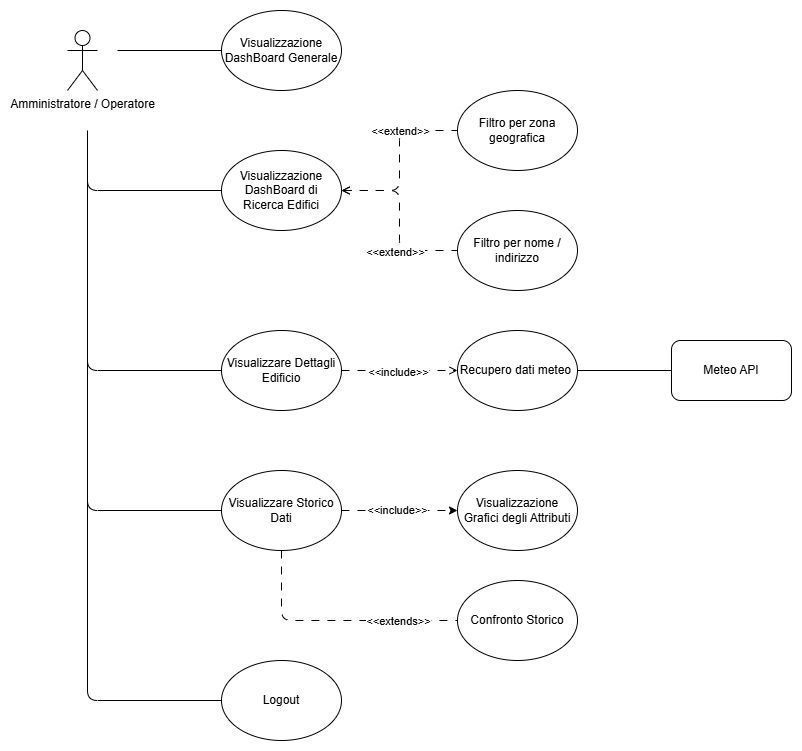
\includegraphics[width=1\textwidth]{../images/UseCase_diagram/useCaseDiagram-USE_CASE4.drawio.png}
        \caption{\textit{Use Case Diagram} - Visualizzazione e Analisi}
    \end{figure}

 \subsection*{\textit{Use Case} RF1: Logout}
        \subsubsection*{Riassunto}
            Questo \textit{Use Case} definisce la sequenza di terminazione sicura della sessione attiva da parte dell'utente loggato, per garantire la confidenzialità dell'accesso alla piattaforma.
        \subsubsection*{Descrizione}
            \begin{enumerate}
                \item L'utente naviga verso la porzione in basso a  destra dello schermo e interagisce con il bottone del profilo cliccando sulla voce di logout nel menù a tendina.
                \item L'architettura chiude la sessione collegata all'account e pulisce i dati in memoria locale.
                \item Completate le procedure di sicurezza, l'applicazione reindirizza l'utente alla schermata di benvenuto forzando la visualizzazione del form di login iniziale.
            \end{enumerate}
        \subsubsection*{Estensioni}
            \begin{enumerate}
                \item \textbf{Scadenza automatica della sessione:} Qualora la validità del token di accesso (8 ore) venga superata, il sistema richiede una nuova autenticazione, bloccando l'accesso alle aree protette.
            \end{enumerate}
    \subsection*{\textit{Use Case} RF2: Visualizzazione Dashboard Generale}
        \subsubsection*{Riassunto}
            Questo \textit{Use Case} illustra come gli utenti, dopo l'accesso, possano visualizzare una una dashboard generale per verificare lo stato e i consumi dei vari edifici monitorati dal sistema.
        \subsubsection*{Descrizione}
            \begin{enumerate}
                \item Dopo aver eseguito il login con successo, l'utente viene indirizzato alla Dashboard generale.
                \item Il backend recupera le letture più recenti. Inoltre calcola le metriche principali (come consumi e stato dei sensori) dell'intera rete per la visualizzazione.
                \item Il frontend utilizza layout grafici intuitivi, visualizzando i consumi energetici totali, numero di sensori attualmente operativi e notifiche non ancora prese in carico.
                \item La pagina ricarica i contenti delle visualizzazioni ogni 90 secondi in maniera trasparente all'utente (senza dover ricaricare la pagina).
            \end{enumerate}
        \subsubsection*{Eccezioni}
            \begin{enumerate}
                \item Nel caso in cui il database non disponga di rilevazioni aggiornate (dovute a un malfunzionamento della rete dei sensori) il sistema mostra all'utente le ultime rilevazioni valide conosciute, accompagnate da un indicatore di stato visibile.
            \end{enumerate}

    \subsection*{\textit{Use Case} RF3: Visualizzazione Dashboard di Ricerca Edifici}
        \subsubsection*{Riassunto}
            Questo \textit{Use Case} documenta il metodo con cui l'utente può esplorare e filtrare il catalogo degli edifici monitorati dal sistema utilizzando vari criteri di ricerca
        \subsubsection*{Descrizione}
            \begin{enumerate}
                \item L'utente si reca presso la pagina degli edifici.
                \item Digita le keyword (come il nome esatto della struttura o il suo indirizzo stradale) all'interno della barra di ricerca o usando gli appositi selettori (per filtrare per tipologia di edificio).
                \item Il sistema interroga il database incrociando i criteri immessi e restituisce i valori pertinenti.
                \item La lista espone le informazioni principali dell'edificio tra cui nome, ubicazione, planimetria e tipologia impianto termico, al fine di consentire una rapida identificazione della struttura cercata.
            \end{enumerate}
        \subsubsection*{Estensioni}
            \begin{enumerate}
                \item \textbf{ Filtro per nome o indirizzo: } Combina più campi per restringere la ricerca e scartare i risultati non pertinenti.
                \item \textbf{Selezione rapida:} Selezionando uno dei risultati dalla griglia, l'utente naviga alla scheda dettagliata dell'edificio corrispondente.
            \end{enumerate}
        \subsubsection*{Eccezioni}
            \begin{enumerate}
                \item Nel caso in cui i criteri immessi non trovino corrispondenza nel database, il sistema impedisce che venga visualizzata una pagina vuota esponendo invece un avviso che invita a rivedere i parametri di ricerca.
            \end{enumerate}

    \subsection*{\textit{Use Case} RF4: Visualizzare Dettagli Edificio}
        \subsubsection*{Riassunto}
            Questo \textit{Use Case} mappa il processo di controllo dei parametri per uno o più edifici pubblici, fornendo un profilo termico completo e aggiornato in tempo reale.
        \subsubsection*{Descrizione}
            \begin{enumerate}
                \item Partendo dalla mappa o dalla maschera di ricerca, l'utente seleziona lo stabile da analizzare.
                \item Il frontend mostra la pagina di dettaglio recuperando dal backend le informazioni principali dell'edificio (denominazione, ubicazione, metratura, anno di posa in opera).
                \item Contemporaneamente, vengono scaricati le misurazioni più recenti dei sensori, permettendo di visualizzare la temperatura (intera o esterna) e il consumo energetico istantaneo.
                \item L'interfaccia propone grafici delle misurazioni salvate oltre a mostrare lo  stato di ciascun hardware installato negli immobili.
            \end{enumerate}
        \subsubsection*{Estensioni}
            \begin{enumerate}
                \item \textbf{Cambio intervallo temporale:} Modifica rapida del periodo analizzato nei grafici, selezionando un intervallo predefinito (ultimi 7, 30, 90 o 365 giorni) oppure tramite la scelta di due date distinte.
                \item \textbf{Zoom grafici:} Possibilità di isolare specifici punti sul grafico, per poter ispezionare il valore della singola misurazione.
            \end{enumerate}
        \subsubsection*{Eccezioni}
            \begin{enumerate}
                \item Nel caso in cui la rete di termometri e contatori dell'edificio risultino offline, la dashboard grafica segnala la problematica tecnica congelando la visualizzazione al momento dell'ultima trasmissione utile.
            \end{enumerate}

    \subsection*{\textit{Use Case} RF4: Visualizzare Storico Dati}
        \subsubsection*{Riassunto}
            Questo \textit{Use Case} descrive le modalità con cui l'utente può selezionare lo spazio temporale per l'analisi delle misurazioni termiche e dei consumi energetici.
        \subsubsection*{Descrizione}
            \begin{enumerate}
                \item Rimanendo sulla pagina di dettaglio, l'utente decide di avviare l'analisi selezionando dal menù un attributo primario da graficare (es: andamento termico, consumo del gas metano, consumo energetico).
                \item L'utente stabilisce l'ampiezza dell'asse temporale impostando la data desiderata.
                \item Il sistema aggiorna il grafico in base all'intervallo temporale scelto.
            \end{enumerate}
        \subsubsection*{Eccezioni}
            \begin{enumerate}
                \item Nel caso in cui il database non contenga misurazioni dell'attributo richiesto nel lasso temporale (ad esempio a causa di sensori non ancora installati in tale data), l'interfaccia restituisce un avviso informando l'utente dell'assenza di dati pertinenti.
            \end{enumerate}

\subsection*{\textit{Use Case} RF8: Monitoraggio in Tempo Reale}
        \subsubsection*{Riassunto}
            Questo \textit{Use Case} descrive il monitoraggio continuo dei dati di un edificio selezionato, con aggiornamento automatico delle letture senza intervento manuale dell'utente.
        \subsubsection*{Descrizione}
            \begin{enumerate}
                \item L'utente, all'interno del dettaglio di un edificio, attiva la vista di monitoraggio in tempo reale dei parametri misurati.
                \item Il sistema recupera periodicamente le letture più recenti (temperatura interna, temperatura esterna, consumo energetico istantaneo) e aggiorna la schermata senza ricaricare la pagina.
                \item L'intervallo di aggiornamento è configurabile tramite le impostazioni di sistema, con un valore predefinito di 90 secondi.
                \item La vista integra le serie storiche delle ultime 24 ore per contestualizzare i valori correnti rispetto all'andamento recente.
            \end{enumerate}
        \subsubsection*{Eccezioni}
            \begin{enumerate}
                \item Nel caso in cui i sensori dell'edificio risultino offline, il sistema mantiene le ultime letture valide disponibili e segnala chiaramente lo stato di disconnessione dei dispositivi.
            \end{enumerate}
\newpage
\subsection{\texorpdfstring{{Amministratore e Operatore Tecnico - Gestione e Configurazione}}{Amministratore e Operatore Tecnico - Gestione e Configurazione}}
    Di seguito i requisiti relativi alla gestione operativa dell'infrastruttura, inclusa l'anagrafica degli edifici, l'hardware IoT e le allerte. Verranno esplorati i seguenti Use Case:
    \begin{itemize}
        \item \textbf{RF5}: Gestione Edifici e Sensori 
        \item \textbf{RF6}: Gestire Notifiche di Allarme
        \item \textbf{RF7}: Visualizzare Stato Sensori  
        \item \textbf{RF9}: Configurare Soglie di Allarme 
    \end{itemize}
    \begin{figure}[H]
        \centering
        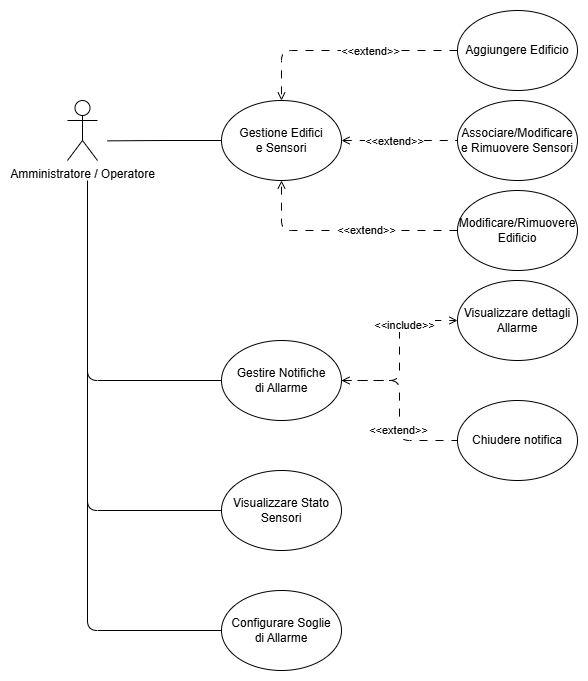
\includegraphics[width=0.8\textwidth]{../images/UseCase_diagram/useCaseDiagram-USE_CASE3.drawio.png}
        \caption{\textit{Use Case Diagram} - Gestione e Configurazione}
    \end{figure}

    \subsection*{\textit{Use Case} RF5: Gestione Edifici e Sensori}
        \subsubsection*{Riassunto}
            Questo \textit{Use Case} descrive come l'utente (Amministratore o Operatore Tecnico) può gestire l'anagrafica completa degli edifici pubblici monitorati e configurare i relativi parametri operativi dei sensori hardware associati a ciascuno stabile.
        \subsubsection*{Descrizione}
            \begin{enumerate}
                \item L'utente accede alla sezione dedicata alla gestione dal menù principale dell'applicazione, visualizzando la lista delle strutture e dei dispositivi.
                \item L'utente può inserire i dati anagrafici fondamentali per registrare un nuovo stabile, specificando nome, indirizzo, superficie e tipologia dell'impianto di riscaldamento.
                \item Successivamente, è possibile mappare e configurare la rete IoT associando, modificando o rimuovendo dispositivi (termometri o contatori), definendone la tipologia esatta e la posizione fisica all'interno delle stanze.
                \item Il sistema valida i dati in ingresso, assicurandosi in particolare dell'univocità del codice identificativo dell'edificio prima di procedere al salvataggio nel database.
                \item Infine, il sistema applica le frequenze di trasmissione dati (media di 90 secondi).
            \end{enumerate}
        \subsubsection*{Estensioni}
            \begin{enumerate}
                \item \textbf{Aggiungere Edificio / Modificare o Rimuovere Edificio:} Flussi secondari per l'alterazione del ciclo di vita anagrafico della struttura immobiliare.
                \item \textbf{Associare/Modificare e Rimuovere Sensori:} Gestione capillare del singolo hardware installato.
                \item \textbf{Calibrazione:} L'utente può avviare la procedura di calibrazione fine di un sensore termico qualora rilevi discrepanze.
            \end{enumerate}
        \subsubsection*{Eccezioni}
            \begin{enumerate}
                \item Nel caso in cui il codice identificativo scelto per l'edificio non sia univoco, il sistema mostra un messaggio di errore e blocca l'operazione di salvataggio.
            \end{enumerate}

    \subsection*{\textit{Use Case} RF6: Gestire Notifiche di Allarme}
        \subsubsection*{Riassunto}
            Questo \textit{Use Case} illustra la procedura attraverso la quale l'utente può visualizzare, analizzare, prendere in carico e chiudere le notifiche di allarme generate in automatico dalla piattaforma in caso di anomalie termiche o sprechi energetici.
        \subsubsection*{Descrizione}
            \begin{enumerate}
                \item L'utente apre il pannello dedicato alle notifiche per prendere visione delle criticità rilevate negli stabili del Comune.
                \item Il sistema elenca le anomalie attive e non ancora risolte, ordinandole cronologicamente in base al timestamp di generazione.
                \item L'utente seleziona un elemento della lista per ispezionare l'edificio coinvolto, la natura dell'anomalia, i valori registrati dai sensori e le soglie violate (inclusione \textit{Visualizzare dettagli Allarme}).
                \item Una volta che l'operatore tecnico è intervenuto fisicamente o da remoto per risolvere il malfunzionamento, agisce sul sistema per chiudere definitivamente l'allerta (estensione \textit{Chiudere notifica}).
                \item Il sistema archivia l'evento nello storico, memorizzando l'identificativo di chi ha validato la chiusura del problema.
            \end{enumerate}
        \subsubsection*{Estensioni}
            \begin{enumerate}
                \item \textbf{Chiudere notifica:} Azione terminale che risolve lo stato di allerta sull'edificio.
            \end{enumerate}
        \subsubsection*{Eccezioni}
            \begin{enumerate}
                \item Nel caso in cui non vi siano allerte attive, il sistema mostra un messaggio appropriato.
            \end{enumerate}

    \subsection*{\textit{Use Case} RF7: Visualizzare Stato Sensori}
        \subsubsection*{Riassunto}
            Questo \textit{Use Case} descrive come l'utente può monitorare in tempo reale lo stato dei sensori installati negli immobili, permettendo che essi riportino misurazioni corrette.
        \subsubsection*{Descrizione}
            \begin{enumerate}
                \item L'utente naviga all'interno dell'elenco completo dei dispositivi di misurazione.
                \item Il sistema, per ogni singolo sensore, permette di visualizzare lo stato di attività (Attivo oppure Offline), la data e l'ora esatta dell'ultimo aggiornamento ricevuto e la posizione fisica registrata.
                \item Il frontend evidenzia i sensori che risultano disconnessi o che non trasmettono dati entro la finestra temporale prevista dalla loro configurazione.
            \end{enumerate}
        \subsubsection*{Estensioni}
            \begin{enumerate}
                \item \textbf{Filtri di visualizzazione:} L'utente può filtrare dinamicamente la lista per stato (mostrando solo gli offline o solo gli attivi), per singolo edificio, per tipo di sensore o tramite query testuale.
            \end{enumerate}

    \subsection*{\textit{Use Case} RF9: Configurare Soglie di Allarme}
        \subsubsection*{Riassunto}
            Questo \textit{Use Case} descrive in che modo l'utente può definire le regole logiche e i parametri limite che comandano l'automazione del sistema di avvisi, per la prevenzione degli sprechi.
        \subsubsection*{Descrizione}
            \begin{enumerate}
                \item L'utente entra nella pagina dedicata alla configurazione delle regole di monitoraggio termico ed energetico.
                \item L'utente procede definendo i range operativi di temperatura inserendo le soglie minime e massime desiderate.
                \item Il sistema aggiorna i parametri di monitoraggio.
            \end{enumerate}
        \subsubsection*{Eccezioni}
            \begin{enumerate}
                \item Nel caso in cui i valori matematici inseriti dall'utente risultino incoerenti (ad esempio la soglia minima inserita risulta maggiore della massima), il sistema blocca il salvataggio e mostra a schermo un messaggio di errore.
            \end{enumerate}
\newpage
\subsection{\texorpdfstring{{Amministratore}}{Amministratore}}
    Di seguito vengono elencati i requisiti associati esclusivamente alla figura dell’Amministratore Comunale, l’unico in possesso dei privilegi necessari alla gestione del personale tecnico e all’esportazione della reportistica.
    \begin{itemize}
        \item \textbf{RF10}: Esportare Dati 
        \item \textbf{RF11}: Gestire Utenti 
        \item \textbf{RF12}: Visualizzare Analisi Comparative 
    \end{itemize}
    \begin{figure}[H]
        \centering
        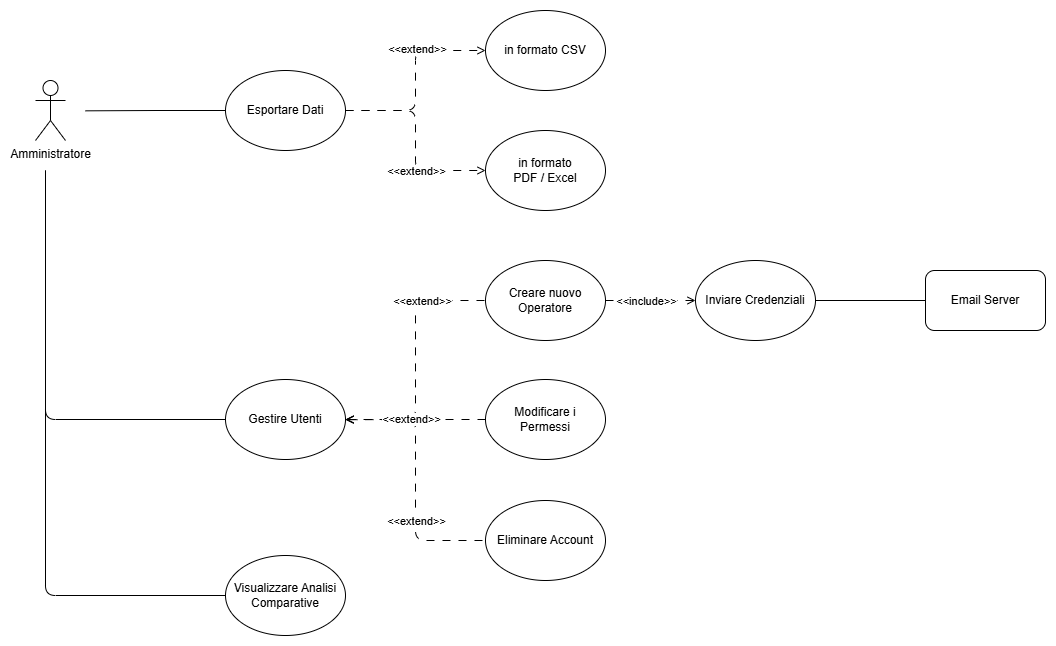
\includegraphics[width=1\textwidth]{../images/UseCase_diagram/useCaseDiagram-USE_CASE5.drawio.png}
        \caption{\textit{Use Case Diagram} - Funzionalità esclusive dell'Amministratore Comunale}
    \end{figure}

    \subsection*{\textit{Use Case} RF10: Esportare Dati}
        \subsubsection*{Riassunto}
            Questo \textit{Use Case} illustra il processo mediante  il quale l’amministratore esegue l’estrazione dei record (consumi ed efficienza) immagazzinati nel database, trasformandoli in file adatti alla rendicontazione o alla manipolazione in fogli di calcolo.

        \subsubsection*{Descrizione}
            \begin{enumerate}
                \item L’amministratore seleziona dal pannello di esportazione un edificio, oppure può selezionarne molteplici per ottenere un file aggregato.
                \item Si seleziona la porzione temporale dei log desiderata (ad esempio, il trimestre invernale passato).
                \item Il software di backend crea un file strutturato assemblando le variabili più importanti come la temperatura ambientale, i chilowattora consumati, i timestamp esatti delle misurazioni e nel caso in cui ci fossere state in quel periodo i registri delle anomalie.
                \item Terminata l’elaborazione, il browser del client salva il file reportistico nel computer locale dell’amministratore.
            \end{enumerate}
        \subsubsection*{Estensioni}
            \begin{enumerate}
                \item \textbf{Formati di output:} Possibilità di scaricare il file in formato CSV (per script automatizzati), o in alternativa PDF ed Excel per una consultazione più user-friendly (Estensioni \textit{in formato CSV}, \textit{in formato PDF/Excel}).
            \end{enumerate}
        \subsubsection*{Eccezioni}
            \begin{enumerate}
                \item Nel caso in cui i filtri temporali non restituiscono dati, il sistema blocca la generazione del file e segnala che non ci sono record da estrarre
            \end{enumerate}

    \subsection*{\textit{Use Case} RF11: Gestire Utenti}
        \subsubsection*{Riassunto}
            Questo \textit{Use Case} definisce come l'amministratore gestisce l'intero ciclo di vita degli account degli operatori tecnici per consentire l'accesso alla rete IoT esclusivamente al personale autorizzato.
        \subsubsection*{Descrizione}
            \begin{enumerate}
                \item L'amministratore accede alla console di sicurezza per gestire l'anagrafica degli account.
                \item Selezionando la volontà di creare una nuova identità (\textit{Creare nuovo Operatore}), compila il form specificando l'indirizzo email aziendale della nuova risorsa e selezionando i privilegi (ruolo) da conferirle.
                \item Il processo esegue un rapido controllo di integrità verificando che la mail indicata non sia già presente nei registri del database.
                \item Superato il controllo, il sistema invoca \textit{Inviare Invito}: l'Email Server invia al tecnico un link univoco per completare la registrazione e impostare la password.
            \end{enumerate}
        \subsubsection*{Estensioni}
            \begin{enumerate}
                \item \textbf{Modificare i Permessi / Eliminare Account:} Flussi alternativi per aggiornare i privilegi degli account attivi o revocare definitivamente l'accesso al personale dimissionario.
            \end{enumerate}
        \subsubsection*{Eccezioni}
            \begin{enumerate}
                \item Se l'email inserita è già associata a un account, il sistema blocca la creazione e mostra un messaggio di errore per evitare duplicati.
            \end{enumerate}

    \subsection*{\textit{Use Case} RF12: Visualizzare Analisi Comparative}
        \subsubsection*{Riassunto}
            Questo \textit{Use Case} chiarisce le dinamiche a disposizione della classe amministrativa per eseguire benchmark di rendimento incrociando i profili termici ed energetici di stabili differenti, con l'obiettivo di rintracciare gli edifici più inefficienti del Comune e assegnare i fondi ai lavori di ristrutturazione.
        \subsubsection*{Descrizione}
            \begin{enumerate}
                \item L'amministratore agisce sull'interfaccia apposita componendo un pool di comparazione, avendo la possibilità di includere fino a un massimo di tre edifici contemporaneamente nell'analisi.
                \item Il sistema elabora grandi moli di dati estrapolando i tassi di consumo reali incrociandoli con l'escursione termica mantenuta dalle caldaie.
                \item I risultati vengono espressi tramite l'uso di grafici a barre o a linee comparative e tabelle dotate di indicatori KPI (Key Performance Indicator), che classificano gli edifici mettendone in risalto pregi e criticità d'isolamento.
            \end{enumerate}
        \subsubsection*{Estensioni}
            \begin{enumerate}
                \item \textbf{Export comparativo:} Completata l'analisi a schermo, l'amministratore può esportare il report in formato PDF da allegare alla documentazione pubblica.
            \end{enumerate}
        \subsubsection*{Eccezioni}
            \begin{enumerate}
                \item Se viene selezionato un solo edificio, il pulsante di generazione dell'analisi rimane disabilitato e il sistema richiede di aggiungerne almeno un secondo per avviare il confronto.
            \end{enumerate}